\documentclass[a4paper,11pt]{article}

\usepackage[latin1]{inputenc}
\usepackage[T1]{fontenc}
\usepackage{bbm} %math chars
\usepackage{amsmath}
\usepackage{indentfirst}
\usepackage{fullpage} %minimizes the default margins
\usepackage{url}
\usepackage{graphicx}
\usepackage[center,footnotesize]{caption} %options des legendes des graphes
\usepackage[section]{placeins} %place les figures d'une section avant le debut de la suivante
\usepackage{subfig} %a) b) c)
\usepackage{fancyvrb}

\title{Exercises - Week 8}
\date{}
\author{Genomics and bioinformatics}

\begin{document}
\maketitle

\noindent This series is about Multiple Sequence Alignment (MSA).

\section{MSA with ClustalW}

\noindent ClustalW is a very popular web-based program for performing progressive multiple sequence alignment. His main homepage is located at http://www.clustal.org, but you can run ClustalW online on several servers on the web: in this exercise we shall use ClustalW2 located in the European Bioinformatics Institute (EBI) server at http://www.ebi.ac.uk/Tools/msa/clustalw2. 

\vspace{10mm}

\begin{figure}[h!]
\centering
\begin{verbatim}
>sequence1
PPGVKSDCAS
>sequence2
PADGVKDCAS
>sequence3
PPDGKSDS
>sequence4
GADGKDCCS
>sequence5
GADGKDCAS
\end{verbatim}
\vspace{-60mm}\hspace{20mm}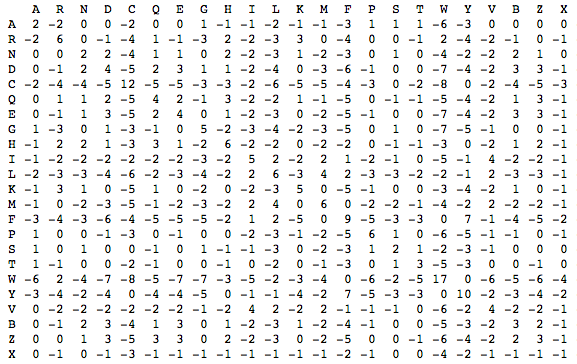
\includegraphics[width=9cm]{PAM250.png}
\caption{The five protein sequences (in FASTA format) and the PAM 250 substitution matrix.}
\end{figure}

\begin{enumerate}
\item Enter these five protein sequences in ClustalW2 with default parameters and click on "Submit".
\item In "Alignments" you will see the MSA found by ClustalW2. 
\item In "Result Summary" the raw alignment scores between all pairwise alignments are shown. Press on "View Output File" to see the total score associated to the MSA. 
\item In "Guide Tree" you can see the tree used to generate the MSA by the progressive alignment method. 
\item Try to change the parameters to see how this affects the MSA.
\item Consider now the PAM 250 scoring matrix (http://www.bioinformatics.nl/tools/pam.html) show in the figure: the value in each cell of a PAM matrix is related to the probability of a column amino acid before the mutation being aligned with a row amino acid afterwards.
Adding a -10 gap penalty, compute the Sum-of-Pair (SP) score of the MSA, by hand or using Python or R [The MSA and PAM250 scoring matrix files can be found on Moodle].
\end{enumerate}
\end{document}











